\documentclass[12pt,a4paper]{article}
\usepackage[utf8]{inputenc}
\usepackage[english]{babel}
\usepackage[T1]{fontenc}
\usepackage{amsmath}
\usepackage{amsfonts}
\usepackage{amssymb}
\usepackage{lmodern}
\usepackage{graphicx}
\usepackage{parskip}
\usepackage{moreverb}

%% Bibliography %%
\usepackage[notlof]{tocbibind}

%% Table %%
\usepackage[table]{xcolor}
\usepackage{array}
\usepackage[hidelinks]{hyperref}

\usepackage{subcaption}
\usepackage{parskip}
\usepackage[top=2.5cm, bottom=2.5cm, left=3cm, right=3cm]{geometry}

%% Header
\usepackage{fancyhdr}
\setlength{\headheight}{15pt}
\pagestyle{fancy}
\fancyhf{}
\rhead{\fancyplain{}{\rightmark }}
\lfoot{\textit{INFO0085-1: Compilers}}
\rfoot{\thepage}
\renewcommand{\footrulewidth}{0.5pt}

%% Color %%
\usepackage{color}
\definecolor{mygrey}{rgb}{0.9, 0.9, 0.9}
\definecolor{mygreen}{rgb}{0, 0.6, 0}
\definecolor{myblue}{rgb}{0, 0, 0.6}

%% Listings %%
\usepackage{listings}
\lstset{
backgroundcolor = \color{mygrey},
language = Python,
frame = single,
basicstyle = \footnotesize,
keywordstyle = \color{myblue},
commentstyle=\color{mygreen},
numbers = left,
numberstyle = \normalsize,
numbersep = 4pt,
}
%%%%%%%%%

%%%%%%%%%%% TITLEPAGE %%%%%%%%%%%%

\author{CATUSANU Paul - EWBANK Tom - VAN DE GOOR Elodie\\s?????? - s102705 - s??????\\1er Master Ing. Civ. Inf.}
\title{INFO0085-1: Compilers}

\begin{document}
\makeatletter
  \begin{titlepage}
  \centering
      {\large \textsc{University of Liège}}\\
      \textsc{Faculty of applied sciences}\\
      \vspace*{0.5cm}
      \hrule
    \vfill    
    	{\LARGE \textbf{Project report:\\}}
    	{\LARGE Development of a compiler\\ for a new programming language}
    \vfill
      
\includegraphics[width=0.6\textwidth]{logo_ulg.png}
     \vfill
      {\large \@title}
    \vfill
    \hrule
        {\large \@author} \\
  \end{titlepage}
\makeatother
%%%%%%%%%%%%%%%%%%%%%%

\tableofcontents
\newpage

\section{Our language: Raccoon}

\paragraph{}
We wanted to have a language easy to understand and used as first language. Our language definition was driven by the python philosophy of “Simple is better than complex” and “Beautiful is better than ugly”. So, we inspired ourselves of the python syntax for much of our language, particularly the indentation to structure the code instead of the punctuation, in order to improve readability.

\paragraph{}
Since our goal is to make a language easy to use for a child who has never programmed before, the Raccoon will have two key particularities:  
 
\begin{itemize}
\item Use of meaningful keywords instead of some usual operators
\item Dynamic typing   
\end{itemize}

\paragraph{}
The features of the Raccoon language are detailed in the following sections.

\subsection{Types}
\paragraph{}
There are five types in Raccoon: Double, Integer, Boolean, List and String.

\paragraph{Numeric types:} All the arithmetic operations, the combinatorial operations and the comparison operations are allowed with those types. When an operation involves different numeric types, the resulting type is considered as Double. Boolean are considered as numeric types, with a value of 1 for "True" and 0 for "False".

\paragraph{Lists:} All the elements of a list must have the same type category (Integer, Double and Boolean are part of the same category, numeric types). The expression to define a list has the form "[\textit{element1, element2,...,elementN}]". The only authorized operations on a list are the access and the modification of its elements. The expression to access or modify an element has the form "\textit{listName}\textbf{[}\textit{index}\textbf{]}" where \textit{index} is an Integer (or an expression leading to one. The index of a list starts at 1. A list is also not allowed to contain other lists.

\paragraph{Strings:} No operations are allowed on Strings. They can only be instantiated and displayed. The expression of a string consist in text surrounded by double quotes. If you want a string to contain the double quotes character, you need to put a backslash right before it. Here is an example:
\begin{verbatim}
str becomes "Our language is called \"Raccoon\""
\end{verbatim}

\subsection{Assignments}

\paragraph{}
An assignment has the form: 
\begin{center}
\textit{variableName}  \textbf{becomes} \textit{expression}
\end{center}

\subsection{Constants}

\paragraph{}
The definition of a constant has the form:
\begin{center}
\textit{constantName} \textbf{is} \textit{expression}
\end{center}

\paragraph{}
A constant can be of any type.

\subsection{Operations}
\paragraph{} 
Raccoon supports the usual operators:

\paragraph{Arithmetic operators:}
+, -, *, /, mod.

\paragraph{Combinatorial operators:}
and, or.

\paragraph{Comparison operators:}
=?, <, <=, >, >=.

\subsection{Indentation}
\paragraph{}
The indentation has to be made of tabulations only, not spaces.

\subsection{Function definition}

\paragraph{}
The definition of a function has the form:

\begin{center}
\textbf{function} \textit{name}\textbf{(}\textit{argument1, argument2,...,argumentN}\textbf{):}
\end{center}
\begin{tabbing}
\hspace{3.5cm} \= \hspace{2cm} \= \kill
   \> \textit{instruction1} \\
   \> \textit{instruction2} \\
   \> ... \\
   \> \textit{instructionN} \\
\end{tabbing}

\paragraph{}
A function has to contain at least one instruction, and of course, the use of a "\textbf{return} \textit{expression}" statement is allowed.

\paragraph{}
Functions doesn't need to be declared before being defined.

\paragraph{}
Arguments are passed by values.

\paragraph{}
Polymorphism is not allowed in Raccoon. It simplifies things and, as this language is intended for young people with no experience in programming, and thus with no intention of building very complex programs, we think that this limitation is not really problematic. 

\subsection{Conditionnals}

\paragraph{}
A conditionnal statement has the form:

\begin{tabbing}
\hspace{5cm} \= \hspace{1cm} \= \kill
   \> \textbf{if} \textit{condition} \textbf{:}  \\  
   \> \> \textit{instruction1} \\
   \> \> \textit{instruction2} \\
   \> \> ... \\
   \> \> \textit{instructionN} \\
   \> \textbf{else if} \textit{condition} \textbf{:} \\
   \> \> \textit{instruction1} \\
   \> \> \textit{instruction2} \\
   \> \> ... \\
   \> \> \textit{instructionN} \\
   \> \textbf{else:} \\
   \> \> \textit{instruction1} \\
   \> \> \textit{instruction2} \\
   \> \> ... \\
   \> \> \textit{instructionN} \\
\end{tabbing}

\paragraph{}
The "\textbf{else if}" and "\textbf{else}" blocks are not mandatory and having more than one "\textbf{else if}" in the same conditionnal is allowed.

\subsection{Loops}

Raccoon provides "while" and "for" loops, along with the special instructions "\textbf{break}" and "\textbf{continue}".

\subsubsection{"while" loop}

\paragraph{}
This loop statement has the form:

\begin{tabbing}
\hspace{5cm} \= \hspace{1cm} \= \kill
   \> \textbf{while} \textit{condition} \textbf{:}  \\  
   \> \> \textit{instruction1} \\
   \> \> \textit{instruction2} \\
   \> \> ... \\
   \> \> \textit{instructionN} \\
\end{tabbing}


\subsubsection{"for" loop}

\paragraph{}
This loop statement has two possible forms:

\begin{tabbing}
\hspace{5cm} \= \hspace{1cm} \= \kill
   \> \textbf{for} \textit{iterator} \textbf{in range(}\textit{start,end}\textbf{):}  \\  
   \> \> \textit{instruction1} \\
   \> \> \textit{instruction2} \\
   \> \> ... \\
   \> \> \textit{instructionN} \\
\end{tabbing}

\paragraph{}
and

\begin{tabbing}
\hspace{5cm} \= \hspace{1cm} \= \kill
   \> \textbf{for} \textit{iterator} \textbf{in} \textit{listName}\textbf{:}  \\  
   \> \> \textit{instruction1} \\
   \> \> \textit{instruction2} \\
   \> \> ... \\
   \> \> \textit{instructionN} \\
\end{tabbing}

\paragraph{}
They work the same as in Python.

\subsection{Scope of variables}

\paragraph{}
The scope of the variables is defined by the function definitions. Each time you enter a new function definition, you enter a new scope. Variables are only accessible in the scope where they were initialized or defined as arguments.

\paragraph{}
However, there is also a particular scope for the variables used as iterator in a "\textbf{for}" loop. The scope of these variables is limited to the "\textbf{for}" block. If a variable was already defined with the same name, this variable is not accessible in the scope of the "\textbf{for}", every uses of this variable inside the "\textbf{for}" statement will refer to the iterator.

\subsection{Comments}

\paragraph{}
Line comments starts with "//" and block comments are delimited by "/*" and "*/". As it was suggested, nested comments are allowed, but have to be correctly used. In other words, all nested block comments that are opened has to closed. Having something like this is correct:
\begin{verbatim}
/* /* where do my comments end? here? */ or here? */
\end{verbatim}
but something like this will generate an error:
\begin{verbatim}
/* /* where do my comments end? here? or here? */
\end{verbatim}


\section{The compiler}

\subsection{Implementation language and tools used}

\paragraph{}
The compiler is written in Python. What motivated us to choose this language is the fact that we found very helpful tools implemented in Python. We have indeed found the website of some informatics teacher named Matthieu Amiguet, who provides a well explained tutorial about the development of a simple compiler, as well as a very handy module which permits to represent and manipulate abstract syntax trees.  

\paragraph{}
The main tool we used in this project, as it is used in Mr. Amiguet's tutorial, is a module called PLY, which is a pure-Python implementation of the popular compiler construction tools lex and yacc.  

\subsection{Development}

\paragraph{}
The implementation of our compiler is separated into five files. One of these files is a modified version of Mr. Amiguet's module "AST.py" for the creation and the handling of abstract syntax trees. The other four files are each responsible for a different step of the compilation process. 

\subsubsection{Lexical analysis}

\paragraph{}
The lexical analysis is implemented in the file "lexical.py".

\paragraph{}
This analysis is divided in two stages. The first stage is aimed at generating a temporary list of tokens, which will then be modified during the second stage in order to take into account the indentation present in the program file that's being analysed.

\paragraph{The first lexing stage:}
This stage simply uses the lex functionality of PLY to generate the list of tokens found in the input file. Among these tokens, the ones called "END\_STATEMENT" contain the informations regarding the indentation. The reason of this is that the pattern for this token matches any new line, along with eventual empty lines and tabulations that follow.

\paragraph{The second lexing stage:}
The role of this stage is to represent the indentation in the token list, using special "INDENT" and "DEDENT" tokens. An occurence of "INDENT" in the list means that every new lines that follows are shifted by a fixed number of tabulations. "DEDENT" cancel the effect of the previous "INDENT" while a new occurence of "INDENT" adds a new shift compared to the previous one. That being said, what this stage do is going through the token list to find the tokens "END\_STATEMENT", deducing the indentation from the tabulations stored in it, and, when necessary, adding new tokens of type "INDENT" and "DEDENT" to the list. The principle of the deduction process is not very complicated, it just requires to keep track of the previous levels of indentation and compare them to the new one.

\paragraph{}
However, with this approach, we coudn't think of a way to include the tokenization of the comments. We thus found a little trick to solve this problem. Instead of passing the original input string to our lexical analyser, we pass a modified version, where all the comments have been removed. We are nonetheless aware that this method is not the most efficient since it requires to go through the whole file one more time.

\paragraph{}
There is still a detail that was needed to make the second lexing stage works. In order to be able to generate the last "END\_STATEMENT" and the right number of "DEDENT" at the end of the token list, the program must end with a "\textbackslash n" character. So, instead of forcing the programmer to end his programs with a new empty line, our compiler just adds it automatically to the input string before starting the analyse.

\paragraph{}
Finally, it is worth mentioning that some error reporting is done during this phase. The lexical analyser will report an error for each illegal character encountered, and for each erroneous level of indentation. By erroneous, we mean that the level of the indentation has decreased, but doesn't correspond to any level of indentation previously encountered. Let's take an example to make things clearer:
\begin{lstlisting}
function example():
		a_fct_call()
	display(something)
\end{lstlisting}
In that case, we got an error at line 3, which should be align either with line 2, either with line 1, but not create a new indentation level between the two. Note that line 3 could also be switched to the right compared to line 2, it is perfectly correct at this stage, but won't be when checking the syntax. The analyser also warns the user if it detects the use of spaces that could corrupt the indentation, but those warnings won't be considered as actual errors, and so they won't prevent the program from being compiled, but it is not a problem, because if the spaces are really corrupting the indentation, the parser will notice it. Those warnings are thus there to provide some additional  information to the error reporting done by the parser, but that topic will be discussed in the next section.
  
\subsubsection{Parsing}

\paragraph{}
The parsing is implemented in the file "parsing.py".

\paragraph{}
The parsing component of PLY is based on Yacc, and Yacc uses the parsing technique known as LR-parsing or shift-reduce parsing. LR parsing is a bottom up technique that tries to recognize the right-hand-side of various grammar rules. Our grammar rules are stated in the docstrings of a series of functions and whenever a valid right-hand-side is found in the input, the code inside the corresponding function is executed and the grammar symbols are replaced by the grammar symbol on the left-hand-side.

\paragraph{}
The grammar, as we implemented it here, is ambiguous. However, the parser can deal with it and inform the user of the actions taken, in the form of 2 messages: "shift/reduce conflicts" or "reduce/reduce conflicts". A shift/reduce conflict is caused when the parser generator can't decide whether or not to reduce a rule or shift a symbol on the parsing stack, and by default, all shift/reduce conflicts are resolved in favor of shifting. In our case, as a matter of fact, this default action solves our ambiguity problems, except for arithmetic or comparison expression rules, which we wrote in this very simple way:
\begin{verbatimtab}[4]
	'''expr : expr ADD_OP expr
			| expr SUB_OP expr
			| expr MUL_OP expr
			| expr DIV_OP expr
			| expr MOD_OP expr
			| expr comb_op expr
			| expr comp_op expr'''
\end{verbatimtab} 
But once again, the Yacc module of PLY provides a way to deal with it. Indeed, it allowed us to define precedence rules for our arithmetic/comparison operators, so that the ambiguity is gone.

\paragraph{}
Of course, this parser is not only responsible for checking the syntax of a Raccoon program, it is also responsible for the building of an abstract syntax tree which will be used during the next steps of the compilation process. That's where the series of functions containing the grammar rules are involved. These functions permits to creates the different nodes of the tree and link them together, according to the rules to which they correspond. As said before, the data structure of the tree is implemented in the module "AST.py", originally written by Matthieu Amiguet,  but specifically adapted to be used with the Raccoon language. The modifications we applied at this stage was the implementation of several subclasses of the basic "Node" class. These subclasses are the different types of node that can compose the abstract syntax tree. As an illustration, the abstract syntax tree generated by our implementation of the QuickSort is shown in figure \ref{quicksort-ast}.

\begin{figure}[ht]
    \center
    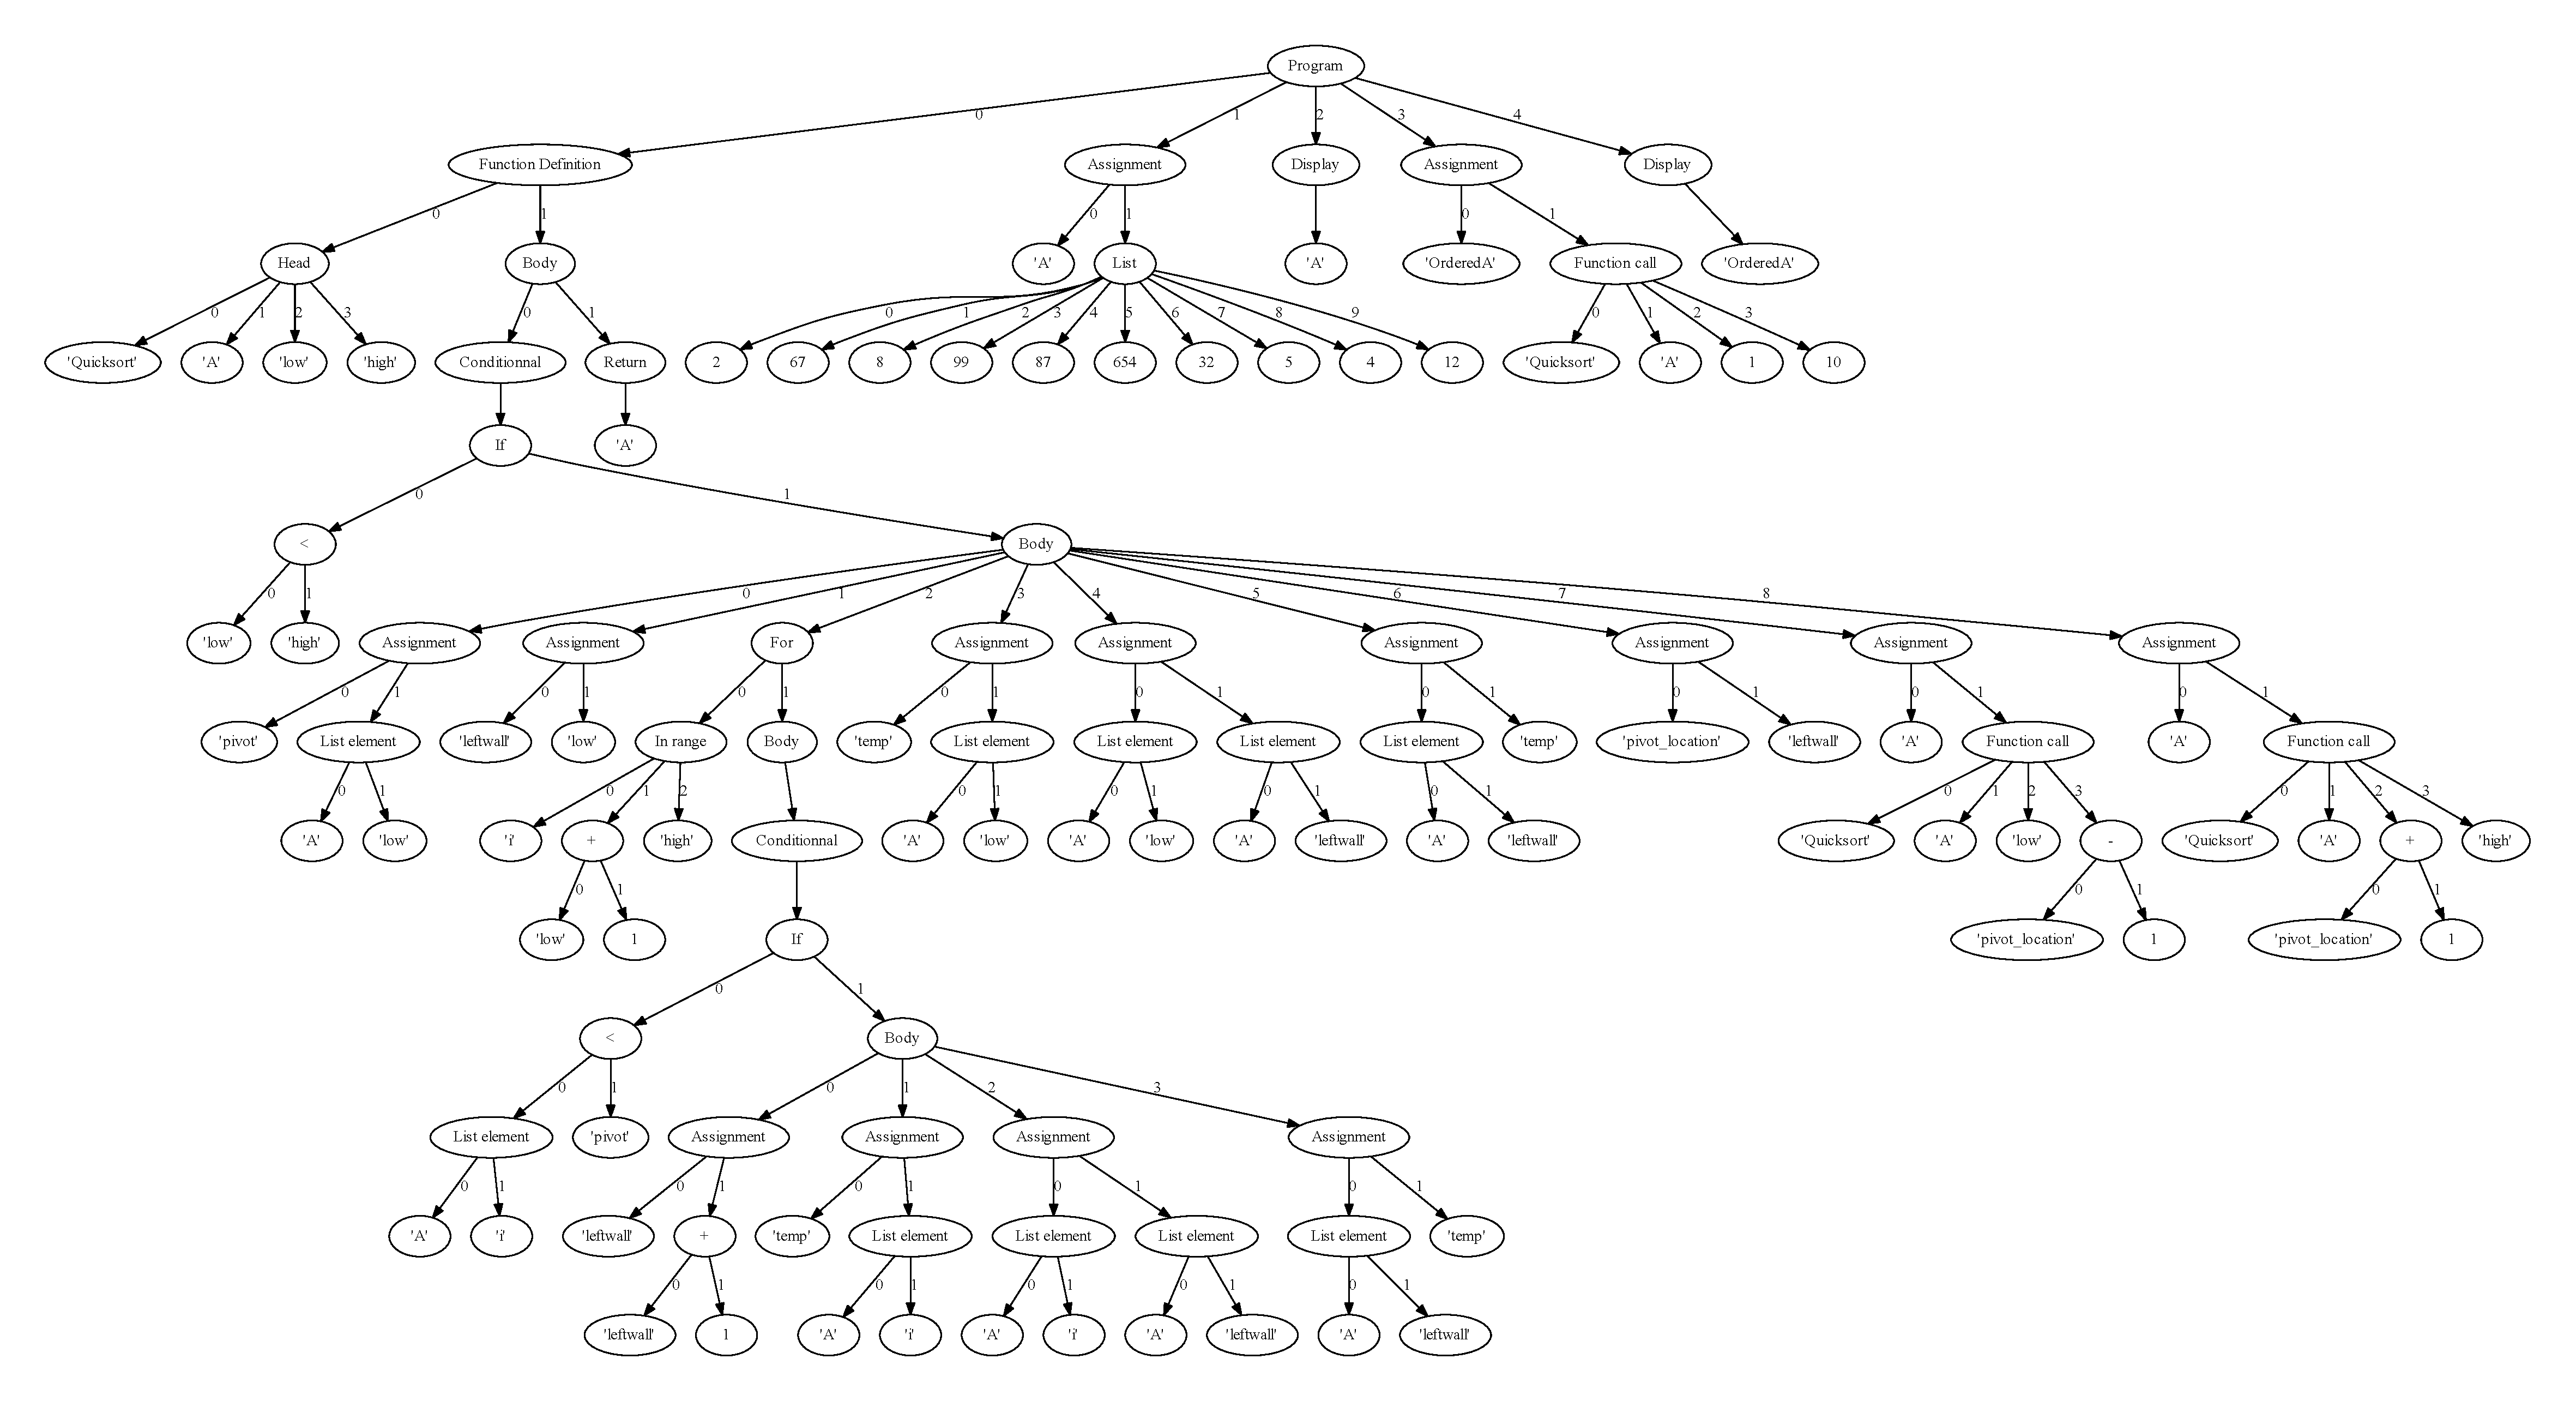
\includegraphics[scale=0.3, angle=90]{figures/QuickSort-ast.pdf}
    \caption{AST of the QuickSort program}
    \label{quicksort-ast}
\end{figure}

\paragraph{}
The last point to address concerning this part is the error reporting. The ideal way of reporting errors would be to have grammar rules for each possible errors, so that the compiler could precisely tell the user what he did wrong. However, that implies that we should think of every possible error cases. So, in order to avoid overloading our grammar with additional rules, and risking leaving bugs in our compiler, we implemented an hybrid solution, which consist in having some grammar rules for the most common errors, and also using what's called a "panic mode recovery". Whenever the panic mode recovery encounters an unknown error, it will first report it, then discard it and restart the parsing from the next token. Because of that, the parser may generate additional errors. So, this is not the perfect solution but, since the Raccoon grammar is not too complicated, we thought that it was sufficient to help the user correcting his mistakes.  

\subsubsection{Semantic analysis}

\paragraph{}
The semantic analysis is implemented in the file "semantic.py". In this module, functions are added to the nodes of the syntax tree, thanks to a decorator. 

\paragraph{}
The first part of these functions permits the "couture" of the AST, allowing a particular traversing of the tree. To sew a node, we first need to sew recursively its children, then the node itself. So, we provided a method to the Node class, that takes as argument the last sewed node, sews the corresponding sub-tree and returns the new "last sewed node". In addition to that, we had to provide a function to start the couture process. This function creates an instance of a special node type, called "EntryNode", which defines the entry point of the program. An example of a sewed tree is given at figure \ref{ast-threaded}, the "couture" is represented by the coloured links.

\begin{figure}[ht]
    \center
    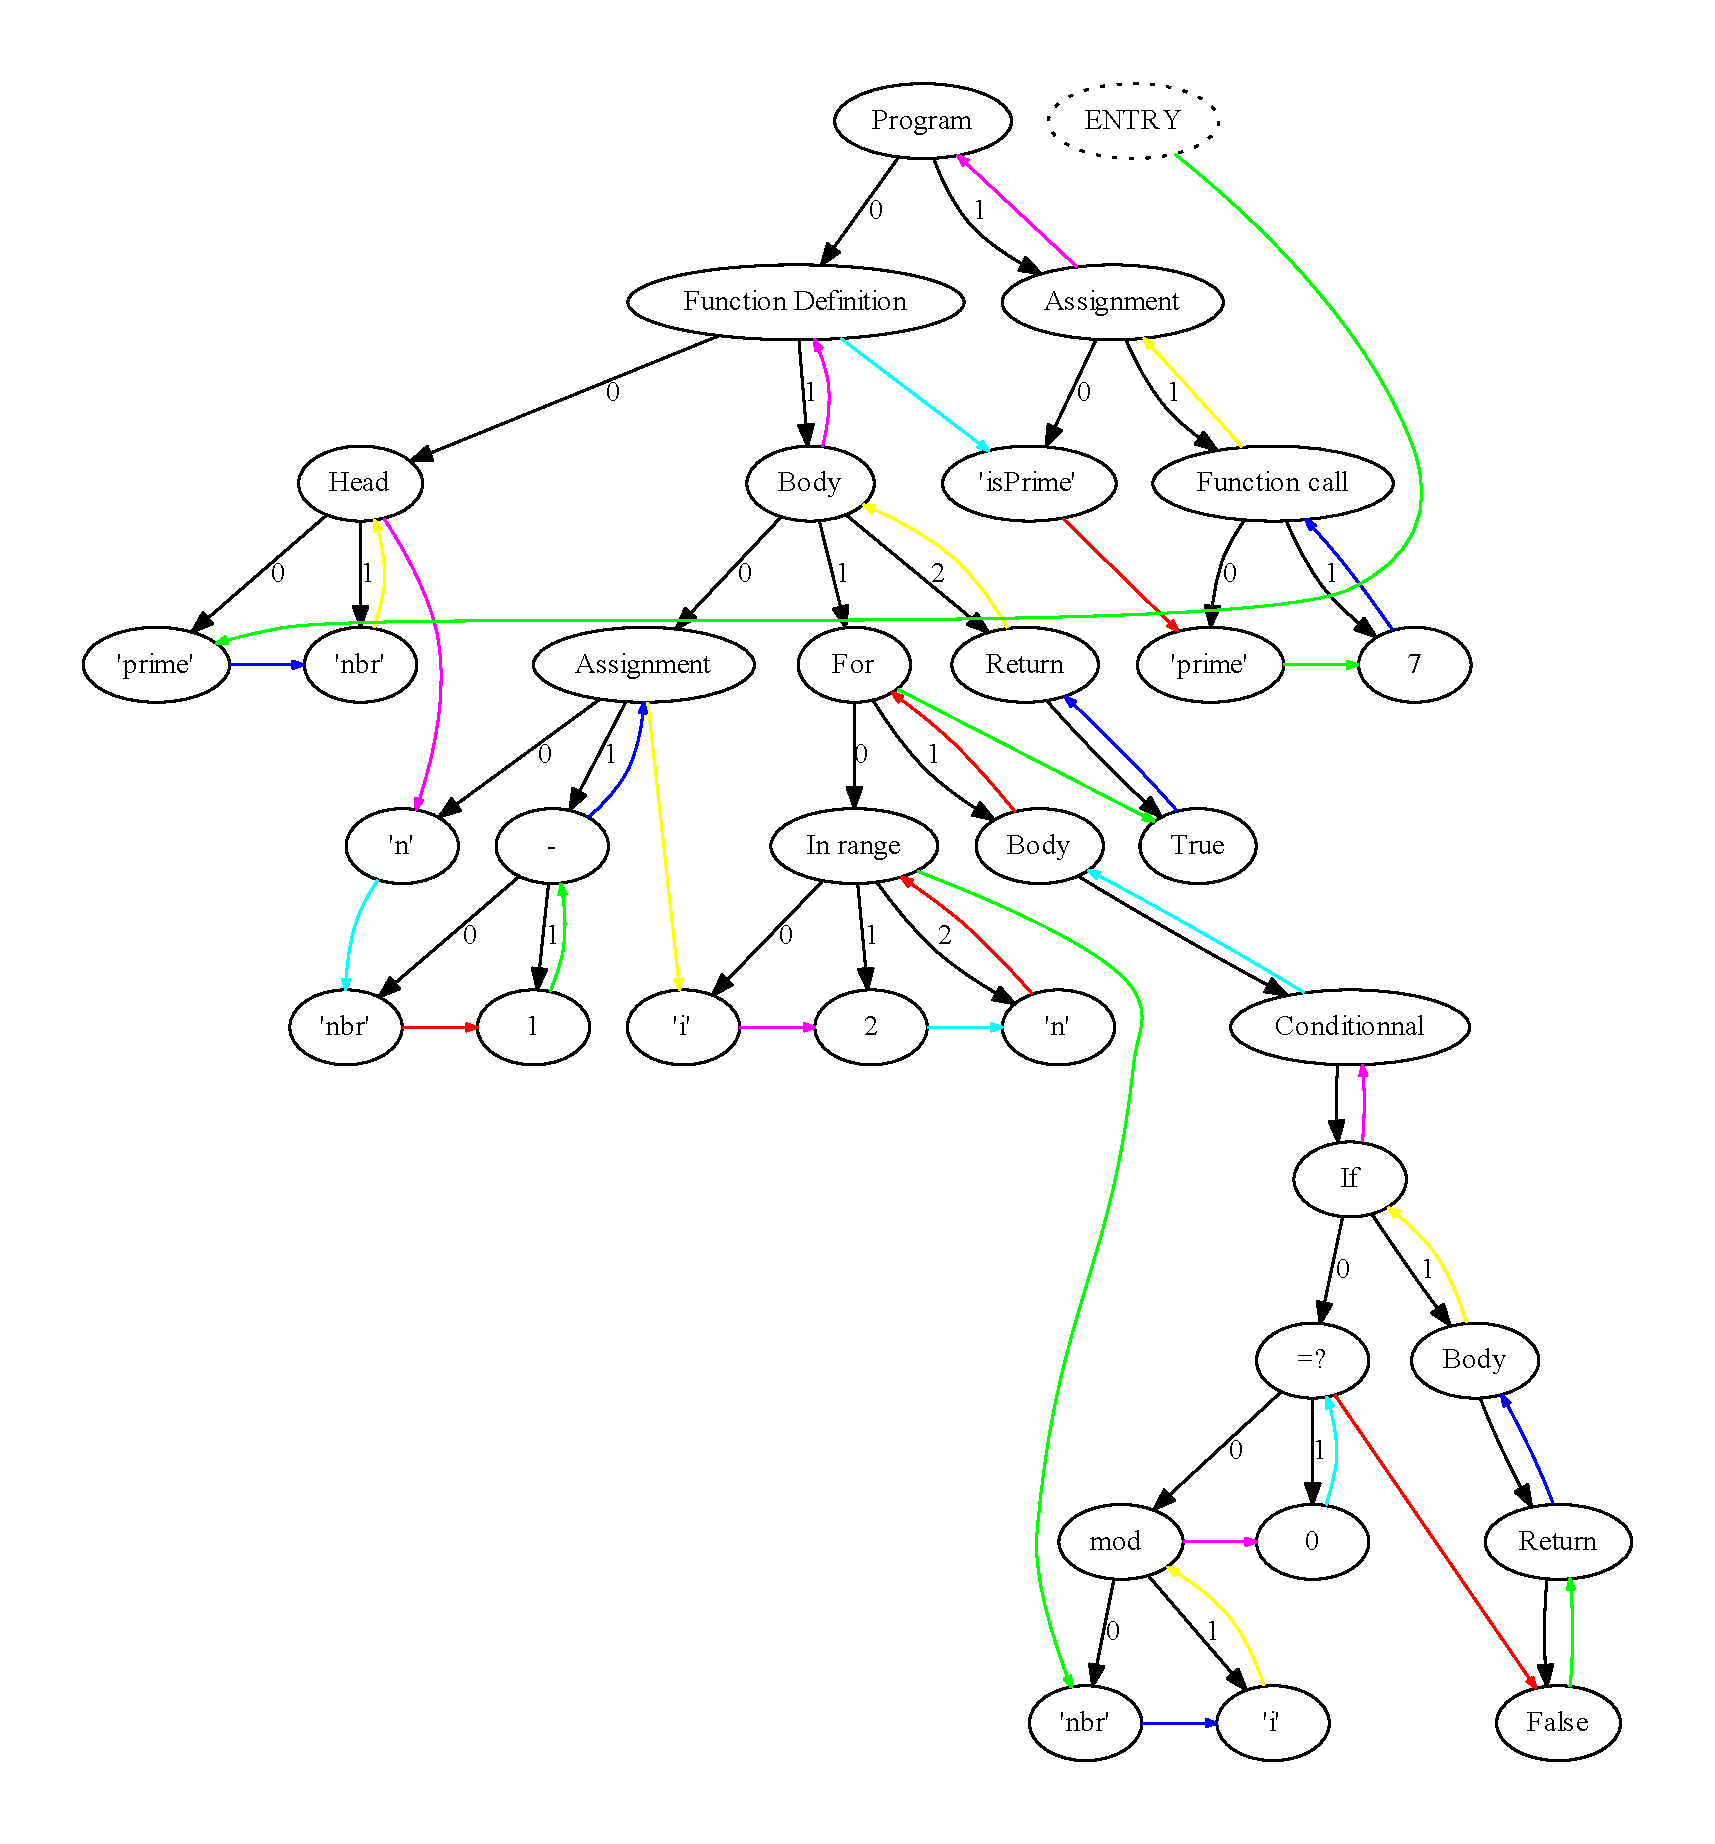
\includegraphics[scale=0.55]{figures/ast-threaded-example.pdf}
    \caption{Couture of an AST}
    \label{ast-threaded}
\end{figure}

\paragraph{}
Once the tree is sewed, we can follow this path and do some semantic checking. This work is done by adding a method "semAnalysis" to each type of node. Each node class has thus its own implementation of this method, because different actions has to be performed depending on the type of node. The only common point to all the nodes is the last instruction of the method, which is of course a call to "semAnalysis" on the next node in the couture.


\paragraph{}
This analysis performs some checking about the following:

\begin{itemize}
\item \textbf{Variables initializations} : each time time an assignment node is encountered, it creates (or modify) an entry in a hash-table. This entry correspond to the name of the variable to which we assign a value, and is associated with the type being assigned. The same happens for the arguments of a function definition, except that this time the types are unknown. That way, each time a variable is used somewhere, we can look up in the hash-table if it was well initialized.

\item \textbf{Functions definitions} : This works the same way as with variables initialisation, with the difference that the information stored along with the name of the function is here the number of arguments. We can then verify if a function call is correct. 

\item \textbf{Types} : Although our language is based on dynamic typing, it is still possible to do some type-checking. Types can be sometimes deduced, and when they can't, we consider them as unknown types which won't interfere with the analysis. The principle here is to keep a stack with the encountered types, and sometimes merge the last two types on the top of stack, for example when an operation node is encountered. This results sometimes in a "forbidden" type, as long as an error report, in case the types are not compatible. This system allows us to report several sorts of erroneous type uses like mixing numeric types with strings, creating list where the elements are not all of the same type, trying to access list elements with something else than an integer,...
Since we were planning on using dynamic typing, we didn't push the thinking too far, but as you will see in the next section, we didn't manage to implement dynamic typing, and we realized too late that maybe it would have been possible to improve this semantic analysis and deduce variable types in every cases.   

\item \textbf{Non context-free statements} : "break" and "continue" instructions has to be used inside a loop, while the "return" statement has to be inside a function definition. This is verified by going trough the parents of the node until it reaches either a loop node or a function definition node, depending on the case. If it reaches the root of the tree before that, it means that the statement is not at the right place.
   
\end{itemize}
  
\paragraph{}
In order to make all these checkings possible, we obviously needed to implement some data structures aimed at containing the type-stack, the hash-tables but also aimed at keeping track of the different scopes of the program. We thus created two new classes in the AST module. The first one represents a scope of the program and contains the hash-tables and the type-stack associated to this scope. The second one maintains a stack whose elements are instances of the previous class. The scope on the top of the stack is the one being manipulated during the analysis. So, each time the semantic analysis enters a new scope, a new "Scope" object is pushed on the stack. Whenever it leaves a scope, it simply pops the last object that was pushed on stack, getting back to the previous scope. This class which handle the stack of scopes is named "ScopeStack" and we instantiates one as a class variable of the "Node" class so that it will be shared by each nodes of the tree. 

\subsubsection{Code generation}

\subsection{How to use}

\subsubsection{Tools installation}
\paragraph{}
First, you need to install PLY. In order to do that, go to the folder "ply-3.4" provided in the project files and run this command:
\begin{verbatim}
C:\...\Raccoon\ply-3.4> python setup.py install
\end{verbatim}

\paragraph{}
Now, to be able to generated graphical representations of abstract syntax trees, you need to install the Graphviz software and the PyDot module. You can get those respectively at \url{http://www.graphviz.org/} and \url{http://code.google.com/p/pydot/}.

\subsubsection{Running the compiler}
\paragraph{}
To launch the compiler, simply run this command, where \textit{file} is the path to the file you want to compile: 
\begin{verbatim}
C:\...\Raccoon\ply-3.4> python llvm.py file
\end{verbatim}
It will generate a file with the LLVM translation of the program. This LLVM code can then be transformed into native code with the LLVM assembler.

\paragraph{}
It is also possible to launch the different parts of the compiler separately. Instead of running the "llvm.py" file, you could run "lexical.py", "parsing.py" or "semantic.py". You can also add the option "-ast" after the file path, to generate a pdf representation of the abstract syntax tree.

\paragraph{}
As required, a series of test files triggering various kinds of errors are provided in the folder "testFiles", along with the correct program files "QuickSort.rac" and "Prime.rac".

\clearpage
\begin{thebibliography}{9}

\bibitem{gueurts}
\url{http://www.montefiore.ulg.ac.be/\~geurts/Cours/compil/2014/compilers-geurts-february2015.pdf}

\bibitem{amiguet}
\url{http://www.matthieuamiguet.ch/pages/compilateurs}

\bibitem{ply}
\url{http://www.dabeaz.com/ply/ply.html}


\end{thebibliography}

\end{document}